\documentclass[11pt, english] {article}
\usepackage{mathpazo}
\usepackage{palatino}
\usepackage[utf8]{inputenc}
\usepackage{hyperref}
\usepackage[authoryear]{natbib}
\usepackage{graphicx}
\usepackage{subcaption}
\graphicspath{ {./Figures/} }
\title{Capstone Applied AI Project Proposal-[Uncertainty Quantification (UQ) for Hyperelastic Composite Material Simulations]\vspace{-2ex}}

\author{
  Turan, Ozgur Taylan\\
  \href{mailto:o.t.turan@tudelft.nl}{\texttt{o.t.turan@tudelft.nl}}
  \and
  Kato, Yuko\\
  \href{mailto:y.kato@tudelft.nl}{\texttt{y.kato@tudelft.nl}}
\vspace{-2ex}}

\begin{document}

  \maketitle
\textbf{RELEVENCE:} \textless Aerospace Engineering \textgreater, \textless Civil Engineering, and Geosciences \textgreater, \textless Mechanical, Maritime and Materials Engineering \textgreater

\section{Background}
Various engineering applications rely on efficient, high-performance materials to overcome design challenges. This high performance can be achieved by engineering micro-heterogenous materials also known as composites. Since the behavior of composites relies heavily on micro-scale interactions between different components, modeling macro-structures with fully represented microscopic geometry is needed. Thus, the standard finite element modeling approach becomes impractical. Computational homogenization, also known as concurrent finite element analysis (FE$^2$), is a method that is employed to model materials with distinct multi-scaled structures (see Figure \ref{fig:fe2}). FE$^2$ employs the concept of embedding a representative volume element (RVE), at each integration point of the macro-scale problem and obtaining the macroscopic constitutive behavior through homogenization, thus bypassing the need to develop a macro-scale constitutive model. Although it succeeds in upscaling the microscopic material behavior to a certain accuracy, the random generation process of the RVEs introduces uncertainty to the obtained macroscopic behavior. In this project, you will investigate the uncertainty caused by the random RVE generation (see Figure \ref{fig:uq} and observe the real problem in Figure 2 of \cite{vandermeer2016}). The uncertainty quantification might help decrease the computational burden of the data-driven methods as well (see \cite{bessa2017}). 

\begin{figure}
\centering
\begin{subfigure}{0.45\textwidth}
    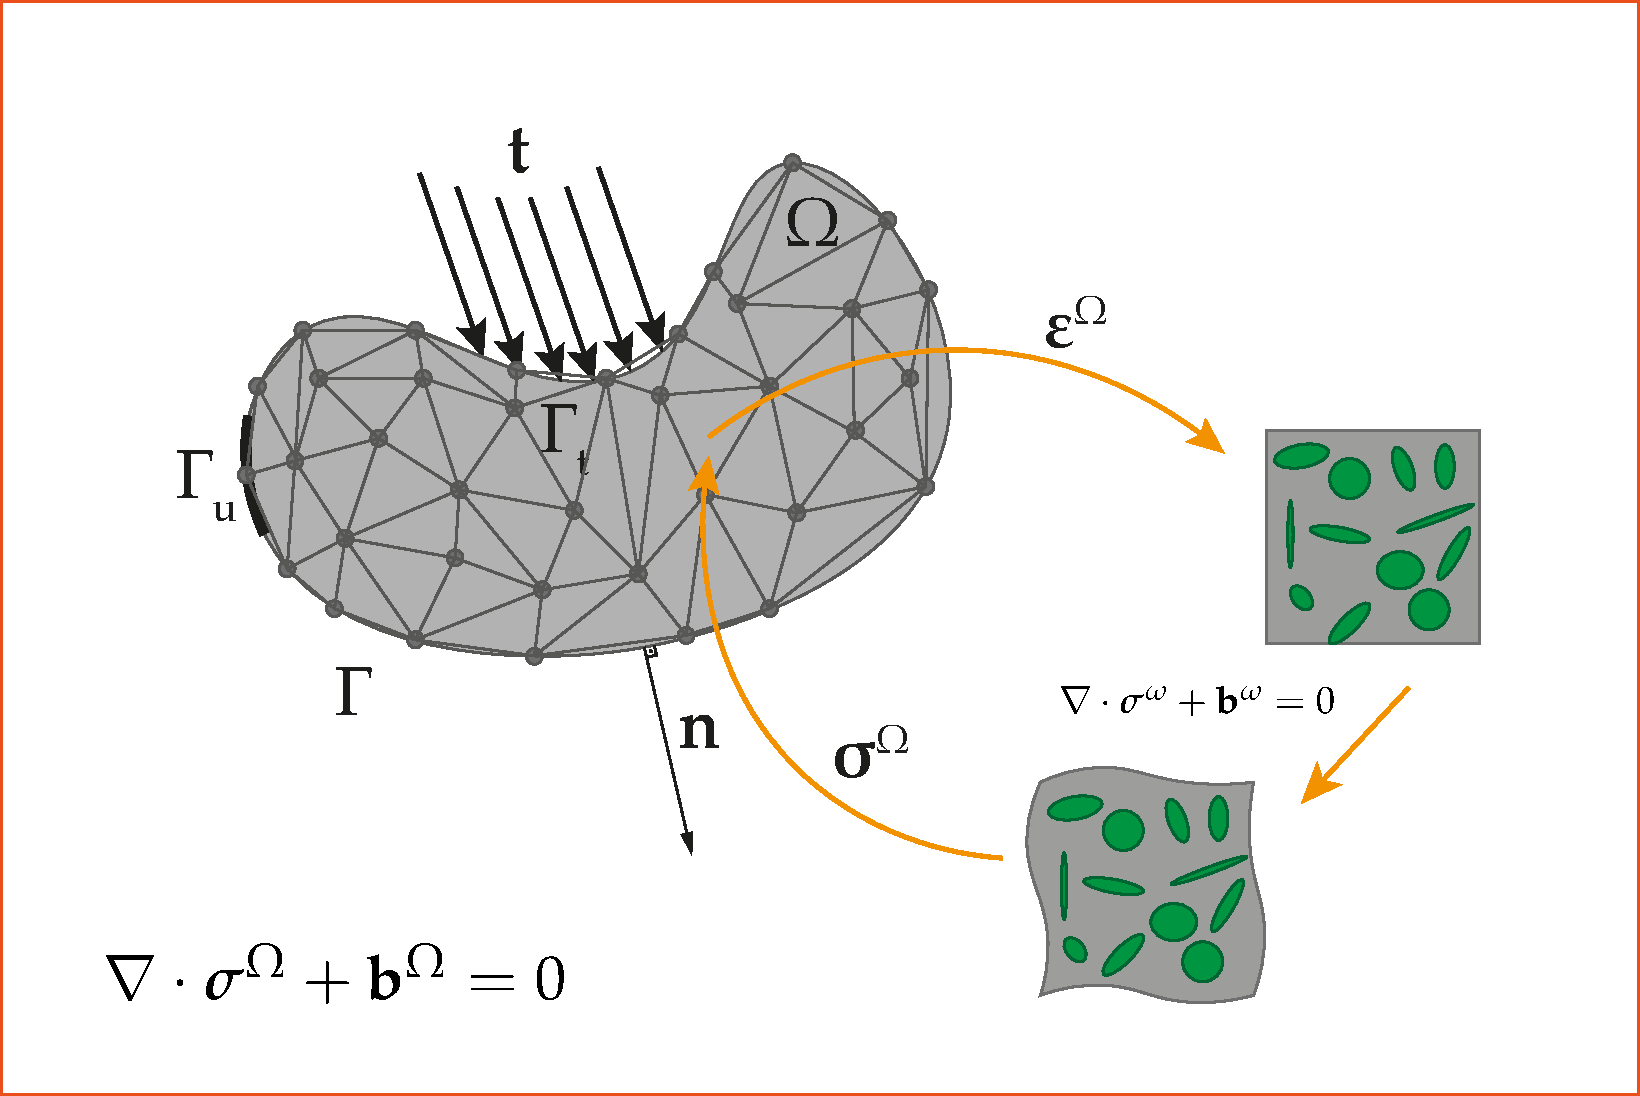
\includegraphics[width=\textwidth]{multiscale}
    \caption{Visualization for FE$^2$.}
    \label{fig:fe2}
\end{subfigure}%
\begin{subfigure}{0.45\textwidth}
    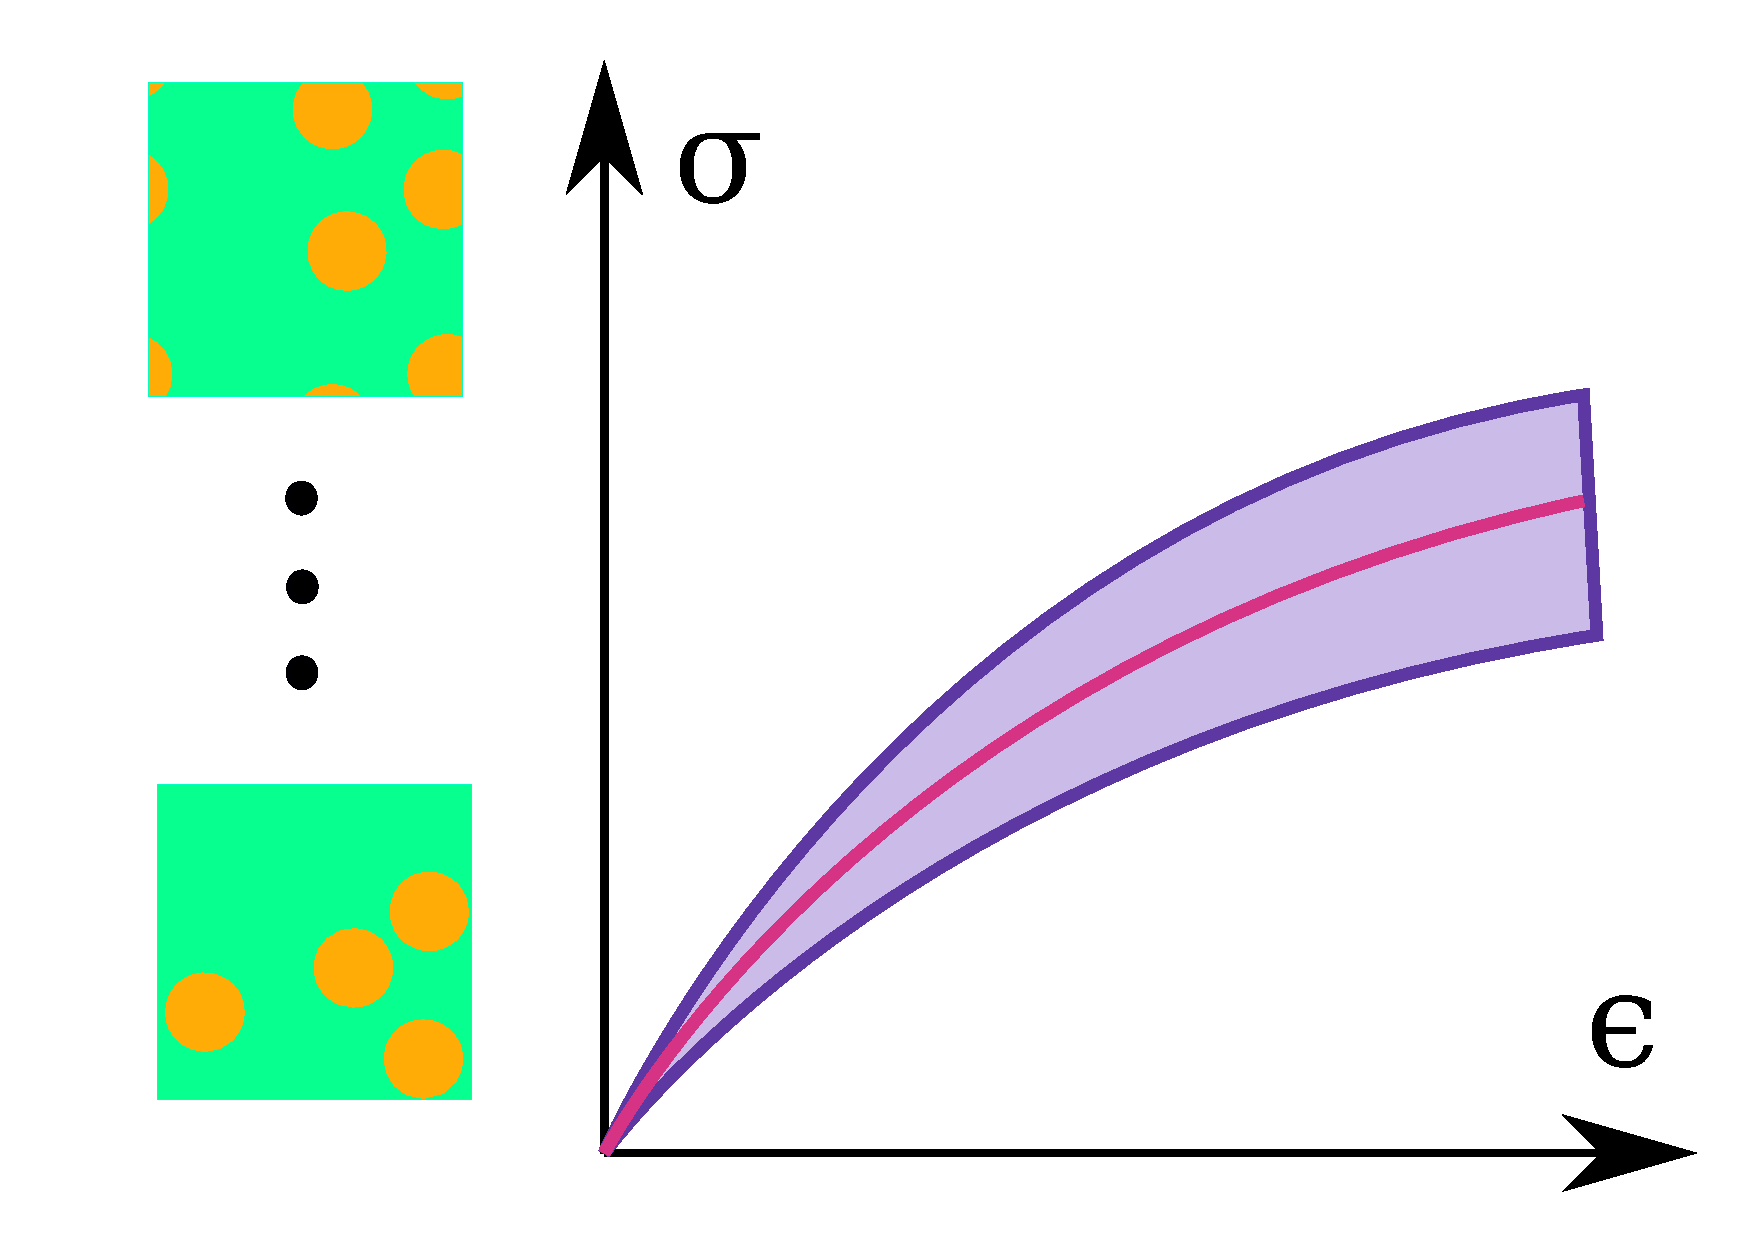
\includegraphics[width=\textwidth]{yuko_aicapstone}
    \caption{Uncertainty caused by micro-structure.}
    \label{fig:uq}
\end{subfigure}
\caption{Background information visualization.}
\label{fig:figures}
\end{figure}

\section{Project Aim}

Students will try to quantify the uncertainty for a heteroscedastic regression problem in 1D and if possible 3D input-output combination.

section{MoSCoW Analysis}
\begin{itemize}
  \item Must understand the cause of the uncertainty in the data, perform UQ for a 1D regression problem with relevant methods and compare them.
  \item Should do a literature review on UQ, 
  \item Could perform the investigation for the 3D $\to$ 3D regression problem.
  \item Won’t be involved in the data generation process.
\end{itemize}

\section{Prerequisites}
\begin{itemize}
  \item Basic knowledge of Finite Element Method (FEM)
  \item Programming experience in Python,
  \item Basic knowledge of Statistics, and Bayesian Machine Learning.
\end{itemize}

\section{AI Approaches and Methods}
\begin{itemize}
  \item Supervised learning 
  \item Uncertainty Quantification
\end{itemize}

\section{Recommended Libraries and Tools}
 \begin{itemize}
  \item NumPy, GPy, pandas, matplotlib, scikit-learn
\end{itemize}

\section{Provided Resources}
  Two types of datasets will be provided from 2D randomly created RVEs. The first one will involve a major directional loading (although the problem is 3D the restriction of a major direction loading makes two other dimensions irrelevant) to create a 1D regression problem. Another optional dataset will be compassed of the 3D regression problem by sampling deformation from Sobol Sequence for the same RVEs that are created.

\bibliographystyle{unsrt}
\bibliography{references/ref.bib}

\end{document}
